% !TeX encoding = UTF-8
% !TeX program = XeLaTeX
% !TeX spellcheck = LaTeX

\documentclass[a4paper]{article}

\usepackage{amsmath,amsfonts,amssymb}
\usepackage{mathrsfs}
\usepackage{bm}
\usepackage{extarrows}
\usepackage{geometry}
\usepackage{ntheorem}
\usepackage{hyperref}
\usepackage[ruled]{algorithm2e}
\usepackage{caption,subcaption}
\usepackage{tikz}

\usetikzlibrary{automata}

\geometry{left=2cm,right=2cm,top=2cm,bottom=2cm}

\def\UrlBreaks{\do\A\do\B\do\C\do\D\do\E\do\F\do\G\do\H\do\I\do\J\do\K\do\L\do\M\do\N\do\O\do\P\do\Q\do\R\do\S\do\T\do\U\do\V\do\W\do\X\do\Y\do\Z\do\[\do\\\do\]\do\^\do\_\do\`\do\a\do\b\do\c\do\d\do\e\do\f\do\g\do\h\do\i\do\j\do\k\do\l\do\m\do\n\do\o\do\p\do\q\do\r\do\s\do\t\do\u\do\v\do\w\do\x\do\y\do\z\do\0\do\1\do\2\do\3\do\4\do\5\do\6\do\7\do\8\do\9\do\.\do\@\do\\\do\/\do\!\do\_\do\|\do\;\do\>\do\]\do\)\do\,\do\?\do\'\do+\do\=\do\#}

\newtheorem{theorem}{Theorem}
\newtheorem{lemma}{Lemma}
\newtheorem{proposition}{Proposition}
\newtheorem{corollary}{Corollary}
\newtheorem{claim}{Claim}
\newtheorem{conjecture}{conjecture}
\newtheorem{definition}{Definition}
\newtheorem{construction}{Construction}
\newtheorem*{proof}{Proof}
\newtheorem*{answer}{Answer}
\newtheorem*{example}{Example}
\newtheorem*{counterexample}{Counterexample}

\newenvironment{exercise}[1]{
	\par
	\noindent\textbf{Exercise #1.}\quad
}{
	\par
	\bigskip
}
\newenvironment{problem}[1]{
	\par
	\noindent\textbf{Problem #1.}\quad
}{
	\par
	\bigskip
}

\DeclareMathAccent{\widehat}{\mathord}{largesymbols}{"62}
\DeclareMathOperator*{\argmax}{\arg\,\max}
\DeclareMathOperator*{\argmin}{\arg\,\min}
\DeclareMathOperator{\E}{\mathbb E}
\DeclareMathOperator{\Var}{\mathrm{Var}}
\DeclareMathOperator{\tr}{\mathrm{tr}}
\DeclareMathOperator{\poly}{\mathrm{poly}}
\newcommand{\abs}[1]{\left| #1 \right|}
\newcommand{\vabs}[1]{\left\| #1 \right\|}
\newcommand{\abra}[1]{\left\langle #1 \right\rangle}
\newcommand{\pbra}[1]{\left( #1 \right)}
\newcommand{\cbra}[1]{\left\{ #1 \right\}}
\newcommand{\sbra}[1]{\left[ #1 \right]}
\newcommand{\floorbra}[1]{\left\lfloor #1 \right\rfloor}
\newcommand{\ceilbra}[1]{\left\lceil #1 \right\rceil}
\newcommand{\bin}{\{0,1\}}
\newcommand{\ZPP}{\mathtt{ZPP}}
\newcommand{\RP}{\mathtt{RP}}
\newcommand{\coRP}{\mathtt{co}\text{-}\mathtt{RP}}
\newcommand{\per}{\text{per}}
\newcommand{\sgn}{\text{sgn}}
\newcommand{\Fbb}{\mathbb{F}}
\newcommand{\Nbb}{\mathbb{N}}
\newcommand{\Rbb}{\mathbb{R}}
\newcommand{\Zbb}{\mathbb{Z}}
\newcommand{\Sset}{\mathbb{S}}
\newcommand{\Fset}{\mathbb{F}}
\newcommand{\Nset}{\mathbb{N}}
\newcommand{\Zset}{\mathbb{Z}}
\newcommand{\Uset}{\mathbb{U}}
\newcommand{\Acal}{\mathcal{A}}
\newcommand{\Bcal}{\mathcal{B}}
\newcommand{\Ccal}{\mathcal{C}}
\newcommand{\Fcal}{\mathcal{F}}
\newcommand{\Gcal}{\mathcal{G}}
\newcommand{\qd}[2]{{\left(\frac{#1}{#2}\right)}}

\bibliographystyle{plainnat}

\title{Exercise Set --- Chapter $4$}
\date{}

\begin{document}

\maketitle

\noindent\textbf{Clarification:} In the following work,
\begin{itemize}
\item if the set of the states of a finite state automaton $A$ is $Q$,
then $Q=\{q_0,q_1,\cdots,q_{|Q|-1}\}$. So $q_t\in Q$ if and only if $t\in\{0,1,\cdots,|Q|-1\}$.
\item if $X\in M_n(\Fset)$, then the subscript of $X_{i,j}$, which means $(i,j)$, goes from $(0,0)$ to $(n-1,n-1)$.
\end{itemize}

\begin{exercise}{4.1.2}\hspace{0pt}\\
    \textbf{e)} $L=\{ww|w\in\{0,1\}^*\}$ is not a regular language.
    \begin{proof}
        Assume $L$ is a regular language and its pumping length is $n$. 
        Consider $w=0^n10^n1$, which is in $L$. By pumping lemma,
        $w=xyz$ where $|xy|\leqslant n,|y|>0$; and $w'=xz$ is also acceptable.
        However, $w'=xz=0^m10^n1,m<n$, contradicting to the definition of $L$.
    \end{proof}
    \textbf{f)} $L=\{ww^R|w\in\{0,1\}^*\}$ is not a regular language.
    \begin{proof}
        Assume $L$ is a regular language and its pumping length is $n$. 
        Consider $w=0^n110^n$, which is in $L$. By pumping lemma,
        $w=xyz$ where $|xy|\leqslant n,|y|>0$; and $w'=xz$ is also acceptable.
        However, $w'=xz=0^m110^n,m<n$, contradicting to the definition of $L$.
    \end{proof}
    \textbf{g)} $L=\{w\overline{w}|w\in\{0,1\}^*\}$ is not a regular language.
    \begin{proof}
        Assume $L$ is a regular language and its pumping length is $n$. 
        Consider $w=0^n1^n$, which is in $L$. By pumping lemma,
        $w=xyz$ where $|xy|\leqslant n,|y|>0$; and $w'=xz$ is also acceptable.
        However, $w'=xz=0^m1^n,m<n$, contradicting to the definition of $L$.
    \end{proof}
    \textbf{h)} $L=\{w1^n|w\in\{0,1\}^*,|w|=n,n\in\Nset\}$ is not a regular language.
    \begin{proof}
        Assume $L$ is a regular language and its pumping length is $n$. 
        Consider $w=0^n1^n$, which is in $L$. By pumping lemma,
        $w=xyz$ where $|xy|\leqslant n,|y|>0$; and $w'=xyyz$ is also acceptable.
        However, $w'=xyyz=0^m1^n,m>n$, contradicting to the definition of $L$.
    \end{proof}
\end{exercise}

\begin{exercise}{4.1.3}\hspace{0pt}\\
    \textbf{a)} $L=\{1w|w\in\{0,1\}^*,(1w)_2\text{ is prime}\}$ is not a regular language.
    \begin{proof}
        Assume $L$ is a regular language and its pumping length is $n$. 
        By \textit{Dirichlet's theorem on arithmetic progressions}, there exists a prime $p$
        of form $2^{n+1}k+1,k\in\Nset^*$. Let $w=xy1$ be its binary expression, where $|y|=n$.
        Also, it is obvious $x>0$.\par
        Since $w=2^{n+1}k+1$, $y$ consists of $n$ zeros.
        By \textit{modified pumping lemma \ref{mpl}},
        $w=xy_1y_2y_31$ and $xy_1y_2^*y_31\in L$. Denote $|y_2|=m$.\par
        Consider $w'=xy_1y_2^{p}y_31$, then $w'$ actually is $2^{n+1+m(p-1)}k+1$.
        Since 
        $$
        2^{n+1+m(p-1)}k+1\equiv (2^{n+1}k+1-1)2^{m(p-1)}+1 \equiv (p-1)2^{m(p-1)}+1\equiv 0\mod p,
        $$
        and $w'>w$, $p$ divides $w'$, thus $w'$ is not a prime,
        contradicting to the definition of $L$.
    \end{proof}
    \textbf{b)} $L=\{0^i1^j|\text{gcd}(i,j)=1\}$ is not a regular language.
    \begin{proof}
        Assume $L$ is a regular language and its pumping length is $n$. 
        Consider $w=0^{(2n)!+1}1^{(2n)!}$, which is in $L$. By pumping lemma,
        $w=xyz$ where $|xy|\leqslant n,|y|=m>0$; and $w'=xyyz$ is also acceptable.
        However, $w'=xyyz=0^{(2n)!+1+m}1^{(2n)!},0<m\leqslant n$ and $2\leqslant 1+m<2n$,
        thus $1+m$ divides $\text{gcd}((2n)!+1+m,(2n)!)$, contradicting to the definition of $L$.
    \end{proof}
\end{exercise}

\begin{exercise}{4.2.2}
    Assume $L$ is a regular language and DFA $A=(Q,\Sigma,\delta,q_0,F)$ accepts $L$.
    Construct DFA $B=(Q,\Sigma,\delta,q_0,F')$, where $q_m\in F'$ if and only if $\delta(q_m,a)\in F$.\par
    As a result, appending an $a$ to any string that ends in $q_m\in F'$ will get to $F$.
    And every string $w\in L/a$ will end in some $q_m\in F'$.
\end{exercise}

\begin{exercise}{4.2.7}
    Assume $L$ is a regular language and DFA $A=(Q,\Sigma,\delta,q_0,F)$ accepts $L$.
    Assume $M$ is a regular language and DFA $B=(Q',\Sigma',\delta',q'_0,F')$ accepts $M$.
    Construct DFA $C=(Q\times Q'\times\{0,1\},\Sigma\cup\Sigma',\hat{\delta},\hat{q}_0,\hat{F})$, where $\hat{q}_0=(q_0,q'_0,0)$, 
    $$
    \hat{F}=\left\{(q_u,q'_v,0)\middle|q_u\in F,q'_v\in F'\right\}.
    $$
    and 
    $$
    \hat{\delta}\left((q_u,q'_v,t),c\right)=\begin{cases}
        (\delta(q_u,c),q'_v,1) & t=0\\
        (q_u,\delta'(q'_v,c),0) & t=1
    \end{cases}.
    $$
    Then $C$ recognizes $\text{alt}(L,M)$ as the third dimension of states controls that 
    only strings with even length may go to 
    accepting states and $C$ reads $w=a_1a_2\cdots a_n$ and $x=b_1b_2\cdots b_n$ by turns.
\end{exercise}

\begin{exercise}{4.2.8}
    Assume $L$ is a regular language and DFA $A=(Q,\Sigma,\delta,q_0,F)$ accepts $L$.
    Define NFA $B=(Q\times Q\times Q,\Sigma,\delta',S,F')$, where 
    \begin{gather*}
        S=\left\{(q_0,q_t,q_t)\middle|q_t\in Q\right\},\\
    \delta'\left((q_u,q_v,q_t),c\right)=\left\{(\delta(q_u,c),q_v,\delta(q_t,c'))\middle|c'\in\Sigma\right\},
    \end{gather*}
    and 
    $$
    F=\left\{(q_u,q_u,q_v)\middle|q_u\in Q,q_v\in F\right\}.
    $$
    Then $B$ recognizes $\text{half}(L)$ as the three dimensions of states shows respectively
    where $w$ ends, where $x$ begins, and where $x$ ends.
\end{exercise}

\begin{exercise}{4.2.9}
    Assume $L$ is a regular language and DFA $A=(Q,\Sigma,\delta,q_0,F)$ accepts $L$.\\
    \textbf{a)} $f(L)=\{w\in\Sigma^*|\exists x\in\Sigma^*,|x|=2|w|,wx\in L\}$
    \begin{proof}
    Define NFA $B=(Q\times Q\times Q,\Sigma,\delta',S,F')$, where 
    \begin{gather*}
    S=\left\{(q_0,q_t,q_t)\middle|q_t\in Q\right\},\\
        \delta'\left((q_u,q_v,q_t),c\right)=\left\{\left(\delta(q_u,c),q_v,\delta(\delta(q_t,c'),c'')\right)\middle|c',c''\in\Sigma\right\},
    \end{gather*}
    and 
    $$
    F=\left\{(q_u,q_u,q_v)\middle|q_u\in Q,q_v\in F\right\}.
    $$
    Then $B$ recognizes $f(L)$ as the three dimensions of states shows respectively
    where $w$ ends, where $x$ begins, and where $x$ ends.
    \end{proof}
    \textbf{b)} $f(L)=\{w\in\Sigma^*|\exists x\in\Sigma^*,|x|=|w|^2,wx\in L\}$
    \begin{proof}
        Let matrix $T\in M_{|Q|}(\Fset_2)$ be the adjacent matrix of $A$, where
        $$
        T_{i,j}=\begin{cases}
            0 & \not\exists c\in\Sigma, \delta(q_i,c)=q_j\\
            1 & \exists c\in\Sigma, \delta(q_i,c)=q_j\\
        \end{cases}.
        $$
        And define the multiplication of two
        matrix $X,Y\in M_{|Q|}(\Fset_2)$ as
        $$
        Z_{i,j}=(XY)_{i,j}=\bigoplus_{k=0}^{|Q|-1} X_{i,k}\otimes Y_{k,j},
        $$
        where
        \begin{figure}[ht!]
          \begin{minipage}[b]{0.5\textwidth}
            \centering
            \begin{tabular}{|c|c|c|} \hline
                $a$ & $b$ & $a\otimes b$\\ \hline\hline
                $0$ & $1$ & $0$ \\ \hline
                $0$ & $0$ & $0$ \\ \hline
                $1$ & $0$ & $0$ \\ \hline
                $1$ & $1$ & $1$ \\ \hline
            \end{tabular}
              \caption*{\textbf{Table $1$:} Operational rule for $\otimes$}
          \end{minipage}%
          \begin{minipage}[b]{0.5\textwidth}
            \centering
            \begin{tabular}{|c|c|c|} \hline
                $a$ & $b$ & $a\oplus b$\\ \hline\hline
                $0$ & $1$ & $1$ \\ \hline
                $0$ & $0$ & $0$ \\ \hline
                $1$ & $0$ & $1$ \\ \hline
                $1$ & $1$ & $1$ \\ \hline
            \end{tabular}
            \caption*{\textbf{Table $2$:} Operational rule for $\oplus$}
          \end{minipage}
        \end{figure}\par
        It is easy to see $(XY)Z=X(YZ)$ and $(T^k)_{i,j}$ actually shows whether there is 
        a path of length $k$ going from $q_i$ to $q_j$.\par
        Define NFA $B=(Q\times Q\times M_{|Q|}(\Fset_2)\times M_{|Q|}(\Fset_2),\Sigma,\delta',S,F')$, where 
        \begin{gather*}
            S=\left\{(q_0,q_t,I,I)\middle|q_t\in Q\right\}\qquad I=\text{diag}\{1,1,\cdots,1\},\\
            \delta'\left((q_u,q_v,X,Y),c\right)=\left\{\left(\delta(q_u,c),q_v,XYT,YT^2\right)\right\},
        \end{gather*}
        and 
        $$
        F=\left\{(q_u,q_u,X,Y)\middle|q_u\in Q,\exists q_v\in F,X_{u,v}=1\right\}.
        $$
        Then $B$ recognizes $f(L)$ as the four dimensions of states shows respectively
        where $w$ ends, where $x$ begins, $T^{n^2}$, and $T^{2n}$. The key idea here is 
        that $(n+1)^2=n^2+2n+1$, so $T^{n^2}$ can be updated during every step;
        and accepting states mean there is a path of length $n^2$ from $q_u$ to somewhere in
        $F$.
    \end{proof}
    \textbf{c)} $f(L)=\{w\in\Sigma^*|\exists x\in\Sigma^*,|x|=2^{|w|},wx\in L\}$
    \begin{proof}
        Same notation with the previous question.\par
        Define NFA $B=(Q\times Q\times M_{|Q|}(\Fset_2),\Sigma,\delta',S,F')$, where 
        \begin{gather*}
            S=\left\{(q_0,q_t,T)\middle|q_t\in Q\right\},\\
            \delta'\left((q_u,q_v,X),c\right)=\left\{\left(\delta(q_u,c),q_v,X^2\right)\right\},
        \end{gather*}
        and 
        $$
        F=\left\{(q_u,q_u,X)\middle|q_u\in Q,\exists q_v\in F,X_{u,v}=1\right\}.
        $$
        Then $B$ recognizes $f(L)$ as the three dimensions of states shows respectively
        where $w$ ends, where $x$ begins, and $T^{2^n}$. The key idea here is 
        that $2^n=2^{n-1}\times 2$, so $T^{2^n}$ can be updated during every step;
        and accepting states mean there is a path of length $2^n$ from $q_u$ to somewhere in
        $F$.
    \end{proof}
\end{exercise}

\begin{exercise}{4.3.2}\hspace{0pt}\\
    \begin{enumerate}
        \item Construct DFA $A=(Q,\Sigma,\delta,q_0,F)$ that accepts $L$. Let $n=|Q|$.
        \item Define matrix $T\in M_{n+1}(\Zset)$ as follows,
            $$
            T_{i,j}=\begin{cases}
                \sum_{c\in\Sigma} [\delta(i,c)=j] & q_i,q_j\in Q\\
                [q_i\in F] & q_i\in Q, j=n\\ 
                [j=n] & i=n\\ 
            \end{cases}.
            $$\par
            It is easy to see that $(T^k)_{i,j},q_i,q_j\in Q$ denotes the number of different
            strings of length $k$ going from $q_i$ to $q_j$;
            and $(T^k)_{i,n},q_i\in Q$ denotes
            the number of different strings of length no more than $k$ going from $q_i$ to
            some $q_t\in F$.
        \item If $L$ accepts at least $100$ strings, let $s_1,s_2,\cdots,s_{100}$ be the 
            shortest $100$ string in $L$. By pumping lemma, $\max_{s_i} |s_i|\leqslant 100n$.\par
            So whether $L$ accepts at least $100$ strings is equivalent to whether 
            the number of different acceptable
            strings of length no more than $100n$ is at least
            $100$, thus equivalent to whether 
            $$
            \left(T^{100n}\right)_{0,n}\geqslant 100.
            $$
    \end{enumerate}
\end{exercise}

\begin{exercise}{4.3.4}\hspace{0pt}\\
    \begin{enumerate}
        \item Construct DFA $A=(Q,\Sigma,\delta,q_0,F)$ accepts
            regular language $L=L_1\cap L_2$.
            The problem is reduced to check whether $A$ accepts any string, including $\varepsilon$. 
        \item DFS from $q_0$ and mark every reachable states.
        \item If some $q_t\in F$ is marked, then $L_1$ and $L_2$ share at least $1$ 
            acceptable string; otherwise, they do not.
    \end{enumerate}
\end{exercise}

\begin{exercise}{4.4.3} 
    The tightest upper bound is $n-2$, which will be obtained under this circumstance:
    \begin{center}
    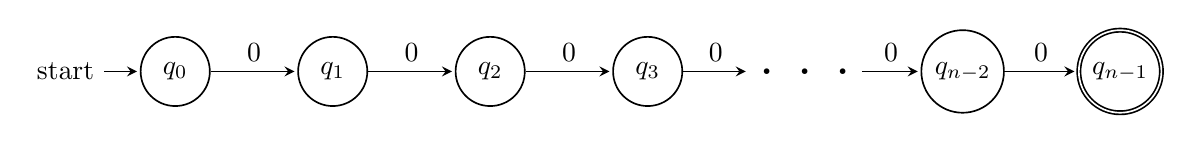
\begin{tikzpicture}[shorten >=1pt,->,>=stealth,semithick,node distance=2cm,auto]
        \node[state,initial] (q0) {$q_0$};
        \node[state] (q1) [right of=q0] {$q_1$};
        \node[state] (q2) [right of=q1] {$q_2$};
        \node[state] (q3) [right of=q2] {$q_3$};
        \node (q4) [right of=q3] {\Huge .\ .\ .};
        \node[state] (q5) [right of=q4] {$q_{n-2}$};
        \node[state,accepting] (q6) [right of=q5] {$q_{n-1}$};

        \foreach \x [remember=\x as \p] in {0,1,...,6}{
            \ifnum \x>0
                \path[->] (q\p) edge node {0} (q\x);
            \fi
        }
    \end{tikzpicture}
    \end{center}
    The shortest string distinguishing $q_0,q_1$ is $0$ repeating $n-2$ times.\par
    The proof that $n-2$ is an upper bound is in Theorem \ref{n-2}.
\end{exercise}


\newpage
\section*{Appendix}

\begin{theorem}[Modified Pumping Lemma]\label{mpl}
Let $L$ be a regular language. Then there exists an integer $p\geqslant 1$
depending only on $L$ such that every string $w=xyz$ in $L$ with  $|y|\geqslant p$
\footnote{$p$ is called the `pumping length'.}
can be written as $w = xy_1y_2y_3z$, satisfying:
\begin{itemize}
\item $|y_2| \geqslant 1$
\item $|y_1y_2| \leqslant p$
\item $xy_1y_2^ny_3z\in L, \forall n \geqslant 0$
\end{itemize}
\begin{proof}
For every regular language there is a finite state automaton $M$ that accepts the language.
The number of states in $M$ is used as the pumping length $p$.\par
Since $|y|\geqslant p$, let $q_0$ be the very state after reading the last character of $x$ and let $q_1, \cdots, q_p$ be the sequence of the next $p$ states.
Because $M$ as only $p$ states, there must be $q_s=q_t,0\leqslant s<t\leqslant p$.
The string read from $q_s$ to $q_t$ is $y_2$, and it naturally separates $y$ to $y_1y_2y_3$.\par
As a result, the multiple occurrence of $y_2$ will be acceptable as well,
therefore $xy_1y_2^ny_3z\in L,\forall n\geqslant 0$.
\end{proof}
\end{theorem}

\begin{theorem}\label{n-2}
    Assume DFA $A=(Q,\Sigma,\delta,q_0,F)$ and $|Q|=n$.
    The shortest string for any two distinguishable states $q_u,q_v$
    is of length no more than $n-2$.
    \begin{proof}
        Let $\Sset_0=F,\Sset_1=Q-F$, so $\forall q_u\in\Sset_0,q_v\in\Sset_1$ the 
        shortest distinguishing string is $\varepsilon$.
        Let $\Sset=\{\Sset_0,\Sset_1\}$ and develop an algorithm as follows:
        \begin{itemize}
            \item \textbf{Step $0$:} Let $\tau(q_t)=\Sset_m,\text{ if }q_t\in\Sset_m$.
            \item \textbf{Step $1$:} If there exists $c\in\Sigma$ and $\Sset_k\in\Sset$ such
                that $\#\{\tau(\delta(q_t,c))|q_t\in\Sset_k\}>1$, go to \textbf{Step $3$};
                otherwise go to \textbf{Step $2$}.
            \item \textbf{Step $2$:} $\Sset$ is the equivalent
                class of distinguishable states. \textbf{Return}.
            \item \textbf{Step $3$:} Let 
                $\Uset=\{\{q_v|q_v\in\Sset_k,\tau(\delta(q_t,c))=\tau(\delta(q_v,c))\}
                |q_t\in\Sset_k\}$.
                Label elements in $\Uset$ as $\Sset_l$ with subscripts never used before,
                then $\Uset=\{\Sset_{l_1},\Sset_{l_2},\cdots,\Sset_{l_t}\}$.
            \item \textbf{Step $4$:} Record the transition with 
                $\eta_1(\Sset_{l_i})=\tau(\delta(q_t,c)),q_t\in\Sset_{l_i}$ and 
                $\eta_2(\Sset_{l_i})=c$.\\
                Update $\Sset$ to $(\Sset-\{\Sset_k\})\cup\Uset$.\\
                Update $\tau(q_t)$ to $\Sset_m,\text{ if }q_t\in\Sset_m,\Sset_m\in\Sset$.\\
                Go to \textbf{Step $1$}.
        \end{itemize}
    This algorithm can be shown as a tree growing. Consider this DFA as an example (the initial state
    is actually irrelevant in the discussion of equivalent states):
    \begin{center}
    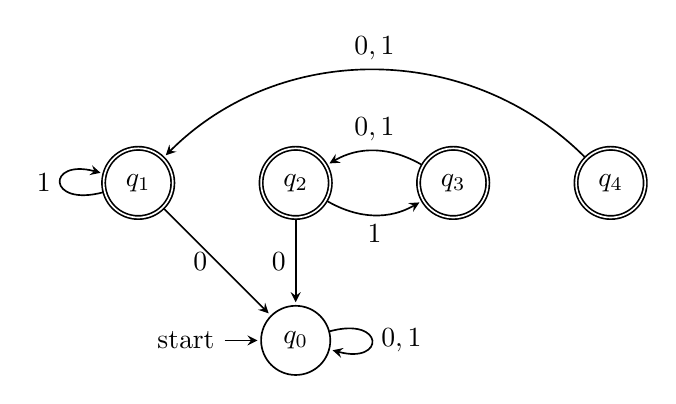
\begin{tikzpicture}[shorten >=1pt,->,>=stealth,semithick,node distance=2cm,auto]
        \node[state,accepting] (q1) {$q_1$};
        \node[state,accepting] (q2) [right of=q1] {$q_2$};
        \node[state,accepting] (q3) [right of=q2] {$q_3$};
        \node[state,accepting] (q4) [right of=q3] {$q_4$};
        \node[state,initial] (q0) [below of=q2] {$q_0$};

        \path[->] (q1) edge[loop left] node {$1$} () edge node[left] {$0$} (q0)
            (q2) edge node[left] {$0$} (q0) edge[bend right] node[below] {$1$} (q3)
            (q3) edge[bend right] node[above] {$0,1$} (q2)
            (q4) edge[bend right=45] node[above] {$0,1$} (q1)
            (q0) edge[loop right] node {$0,1$} ();
    \end{tikzpicture}
    \end{center}
    And the algorithm goes like
    \begin{center}
    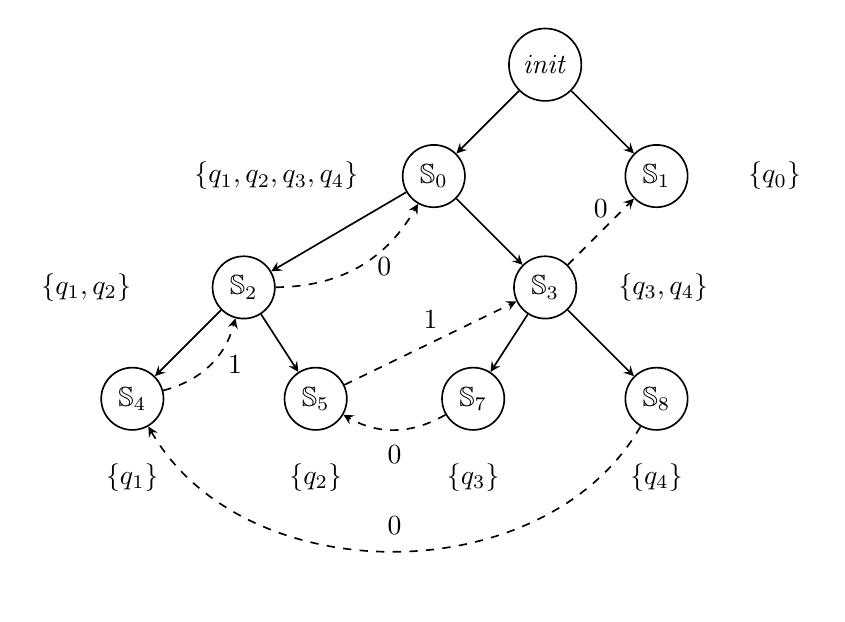
\begin{tikzpicture}[node distance=2cm,semithick,circle,->,>=stealth]
        \node[draw] (q0) {\textit{init}};
        \node[draw] (q1) [below left of=q0] {$\Sset_0$};
        \node (q1') [left of=q1] {$\{q_1,q_2,q_3,q_4\}$};
        \node[draw] (q2) [below right of=q0] {$\Sset_1$};
        \node (q2') [right of=q2,xshift=-5mm] {$\{q_0\}$};
        \node[draw] (q3) [below left of=q1,xshift=-1cm] {$\Sset_2$};
        \node (q3') [left of=q3] {$\{q_1,q_2\}$};
        \node[draw] (q4) [below right of=q1] {$\Sset_3$};
        \node (q4') [right of=q4,xshift=-5mm] {$\{q_3,q_4\}$};
        \node[draw] (q5) [below left of=q3] {$\Sset_4$};
        \node (q5') [below of=q5,yshift=1cm] {$\{q_1\}$};
        \node[draw] (q6) [below right of=q3,xshift=-5mm] {$\Sset_5$};
        \node (q6') [below of=q6,yshift=1cm] {$\{q_2\}$};
        \node[draw] (q7) [below left of=q4,xshift=5mm] {$\Sset_7$};
        \node (q7') [below of=q7,yshift=1cm] {$\{q_3\}$};
        \node[draw] (q8) [below right of=q4] {$\Sset_8$};
        \node (q8') [below of=q8,yshift=1cm] {$\{q_4\}$};

        \path[->] (q0) edge (q1) edge (q2)
            (q1) edge (q3) edge (q4)
            (q3) edge (q5) edge (q6)
            (q4) edge (q7) edge (q8);
        %\draw[->,dashed] (q1) edge[bend left] node[left] {$\varepsilon$} (q0);
        %\draw[->,dashed] (q2) edge[bend right] node[right] {$\varepsilon$} (q0);
        \draw[->,dashed] (q3) edge[bend right] node[right] {$0$} (q1);
        \draw[->,dashed] (q4) edge node[yshift=3mm] {$0$} (q2);
        \draw[->,dashed] (q5) edge[bend right] node[right] {$1$} (q3);
        \draw[->,dashed] (q6) edge node[yshift=3mm] {$1$} (q4);
        \draw[->,dashed] (q7) edge[bend left] node[below] {$0$} (q6);
        \draw[->,dashed] (q8) edge[bend left=60] node[above] {$0$} (q5);
    \end{tikzpicture}
    \end{center}
    Those dashed lines are $\eta_1$ function and the label along the line is $\eta_2$ function.
    Apparently, the transitions go with the order $\Sset_0,\Sset_2,\Sset_3$.\par
    It is easy to see that $\#\{\text{transition}\}=\#\{\text{non-leaf node}\}-1$.
    Since the out-degree of every non-leaf nodes is at least $2$ and $\#\{\text{leaf node}\}\leqslant n$,
    $\#\{\text{transition}\}\leqslant n-2$.\par
    So one distinguishing string for $q_u,q_v$ in different leaf nodes can be constructed as follows:
    \begin{itemize}
        \item \textbf{Step $0$:} Find the leaf nodes $\Sset_k,\Sset_l$ such that $q_u\in\Sset_k,q_v\in\Sset_l$.\\
            Let $w=\varepsilon$.
        \item \textbf{Step $1$:} If the LCA of $\Sset_k,\Sset_l$ is \textit{init}, go to \textbf{Step $2$};\\
            otherwise let the LCA be $\Sset_t$ and go to \textbf{Step $3$}. 
        \item \textbf{Step $2$:} $w$ is the distinguishing string for $q_u,q_v$. \textbf{Return}.
        \item \textbf{Step $3$:} Assume $\Sset_k\subset\Sset_{t_1},
            \Sset_l\subset\Sset_{t_2}$, where $\Sset_{t_1},\Sset_{t_2}$ are different child nodes of $\Sset_t$.\\
            Append $w$ with $\eta_2(\Sset_{t_1})$.\\
            Update $\Sset_k,\Sset_l$ to $\eta_1(\Sset_{t_1}),\eta_1(\Sset_{t_2})$ respectively.\\
            Go to \textbf{Step $1$}.
    \end{itemize}
    The correctness is obvious. Since the append operation occurs with transition function $\eta_1,\eta_2$,
    $|w|\leqslant\#\{\text{transition}\}\leqslant n-2$.
    \end{proof}
\end{theorem}

\end{document}
